%%% LaTeX Template: Two column article
%%%
%%% Source: http://www.howtotex.com/
%%% Feel free to distribute this template, but please keep to referal to http://www.howtotex.com/ here.
%%% Date: February 2011

%%% Preamble
\documentclass[	DIV=calc,%
							paper=a4,%
							fontsize=12pt,%
							onecolumn]{scrartcl}	 					% KOMA-article class

\usepackage{lipsum}													% Package to create dummy text
\usepackage[brazil]{babel}										% English language/hyphenation
\usepackage[protrusion=true,expansion=true]{microtype}				% Better typography
\usepackage{amsmath,amsfonts,amsthm}					% Math packages
\usepackage[pdftex]{graphicx}									% Enable pdflatex
\usepackage[svgnames]{xcolor}									% Enabling colors by their 'svgnames'
\usepackage[hang, small,labelfont=bf,up,textfont=it,up]{caption}	% Custom captions under/above floats
\usepackage{epstopdf}												% Converts .eps to .pdf
\usepackage{subfig}													% Subfigures
\usepackage{booktabs}												% Nicer tables
\usepackage{fix-cm}													% Custom fontsizes
\usepackage[utf8]{inputenc}
\usepackage[top=2.5cm, bottom=2.5cm, left=2.5cm, right=2.5cm]{geometry}
\usepackage[ddmmyyyy]{datetime}
\addto\captionsenglish{%
	\renewcommand\tablename{Tabela}
	\renewcommand\figurename{Figura}
} 
 

 
%%% Custom sectioning (sectsty package)
\usepackage{sectsty}													% Custom sectioning (see below)
\allsectionsfont{%															% Change font of al section commands
	\usefont{OT1}{phv}{b}{n}%										% bch-b-n: CharterBT-Bold font
	}

\sectionfont{%																% Change font of \section command
	\usefont{OT1}{phv}{b}{n}%										% bch-b-n: CharterBT-Bold font
	}



%%% Headers and footers
\usepackage{fancyhdr}												% Needed to define custom headers/footers
	\pagestyle{fancy}														% Enabling the custom headers/footers
\usepackage{lastpage}	

% Header (empty)
\lhead{}
\chead{}
\rhead{}
% Footer (you may change this to your own needs)

%% ====================================
%% ====================================
%% mude o rodape  do projeto
%% ====================================
%% ====================================

\lfoot{\footnotesize \texttt{Cabeamento estruturado} \textbullet ~Modelo de projeto}


\cfoot{}
\rfoot{\footnotesize página \thepage\ de \pageref{LastPage}}	% "Page 1 of 2"
\renewcommand{\headrulewidth}{0.0pt}
\renewcommand{\footrulewidth}{0.4pt}



%%% Creating an initial of the very first character of the content
\usepackage{lettrine}
\newcommand{\initial}[1]{%
     \lettrine[lines=3,lhang=0.3,nindent=0em]{
     				\color{DarkGoldenrod}
     				{\textsf{#1}}}{}}



%%% Title, author and date metadata
\usepackage{titling}															% For custom titles

\newcommand{\HorRule}{\color{DarkGoldenrod}%			% Creating a horizontal rule
									  	\rule{\linewidth}{1pt}%
										}

\pretitle{\vspace{-30pt} \begin{flushleft} \HorRule 
				\fontsize{50}{50} \usefont{OT1}{phv}{b}{n} \color{DarkRed} \selectfont 
				}

\title{Projeto de cabeamento estruturado para biblioteca de universidade}					% Title of your article goes here

%% ====================================



\posttitle{\par\end{flushleft}\vskip 0.5em}

\preauthor{\begin{flushleft}
					\large \lineskip 0.5em \usefont{OT1}{phv}{b}{sl} \color{DarkRed}}
\author{Matheus Garcia Bessegato}  	% Author name goes here


\postauthor{\footnotesize \usefont{OT1}{phv}{m}{sl} \color{Black} 
					\\Universidade Tecnológica Federal do Paraná - Câmpus Cornélio Procópio 								% Institution of author
					\par\end{flushleft}\HorRule}

\date{}																				% No date




%%% Begin document
\begin{document}
\maketitle
\thispagestyle{fancy} 	
\thispagestyle{empty}		% Enabling the custom headers/footers for the first page 
% The first character should be within \initial{}




%% ====================================
%% ====================================
%% mude o resumo  do projeto
%% ====================================
%% ====================================
\initial{O}\textbf{ presente documento descreve o projeto de cabeamento estruturado de uma biblioteca para uma universidade fictícia, que será chamada de UFOPR (Universidade Fictícia do Oeste do Paraná). O corrente projeto parte de uma proposta de planta física para a biblioteca e busca apresentar a elaboração da planta lógica, com todos os equipamentos passivos e ativos da rede, levantamento de quantidades e custo, plano de certificação da rede e orçamento, com base nos usuários e atividades que serão desenvolvidas no ambiente.}

%% ====================================
\begin{figure}
	\centering
	
\includegraphics{utfpr}
\end{figure}

\vspace{3cm}
\centerline{\textit{\textbf{\today}}}

\clearpage
    \renewcommand*\listfigurename{Lista de figuras}
\listoffigures

\renewcommand*\listtablename{Lista de tabelas}
\listoftables




\clearpage
\renewcommand{\contentsname}{Sumário}
\tableofcontents
\clearpage

%% ====================================
%% ====================================
%% Inicio do texto
%% ====================================
%% ====================================
\section{Introdução}
A UFOPR é uma instituição fictícia localizada na região oeste do Paraná que conta com aproximadamente 800 alunos e 120 funcionários, entre professores e técnicos administrativos.

A instituição conta com uma biblioteca provisória, funcionando em um ambiente pequeno e que não atende às demandas da comunidade acadêmica, e planeja construir um novo espaço, adequado para incentivar e dar conforto aos estudos de seus alunos.

O espaço atual da biblioteca conta com apenas 3 computadores para uso dos alunos, 2 ramais VoIP e 6 computadores para os funcionários da mesma. Há instalado no local um switch 10/100 de 24 portas gerenciável para oferecer acesso à Internet no ambiente e não há acesso sem fio.

O novo ambiente contará com uma sala de estudos com 20 computadores e 8 computadores para funcionários, além de acesso sem fio à Internet e 4 ramais VoIP. O ambiente será monitorado por 8 câmeras IP internas.

O atual parque tecnológico da universidade conta com ao menos um computador para cada funcionário, um computador por sala de aula, 6 laboratórios com 41 computadores cada, cobertura Wi-Fi em todo o ambiente administrativo, salas de professores, laboratórios e em salas de aula, monitoramento com 60 câmeras IP e telefonia VoIP com 120 ramais. Os switches são todos gerenciáveis, 10/100 ou 10/100/1000, com divisões em VLANs. O Data Center conta com dois racks de 42U, dois switches CISCO 3750x, Distribuidor Interno Óptico (DIO), um link de dados de 40Mbps e um link de dados de 100Mbps, um Storage NetApp com duas gavetas de expansão, com capacidade de armazenamento aproximada de 50TB e 6 servidores Dell virtualizados, destinados a prover os serviços de impressão, \textit{Active Directory}, \textit{gateway}, antivírus, VoIP, sistema de monitoramento de câmeras, ambiente de ensino a distância, dentre outros.

O presente projeto abrange o estado atual da biblioteca da universidade, as necessidades para a nova biblioteca, seu projeto físico e lógico, um memorial descritivo dos equipamentos passivos que serão utilizados, planilha de orçamentos de materiais, cronograma de implantação, plano de certificação e plano de manutenção.

\subsection{Benefícios}
A execução desse projeto trará maior conforto para os usuários e colaboradores da biblioteca da universidade, bem como deve melhorar a qualidade da aprendizagem, com o aumento do número de computadores para estudo e a oferta de rede sem fio para a conexão com equipamentos pessoais. A concorrência por espaço e equipamentos será menor ou inexistente e a qualidade do serviço oferecido será aprimorada.

\section{Estado atual}
A rede da atual biblioteca conta com:

\begin{itemize}
	\item 01 \textit{patch panel} de 24 portas Furukawa categoria 5e;
	\item cabeamento Furukawa categoria 5e;
	\item 01 switch CISCO 10/100 gerenciável de 28 portas;
	\item 01 rack de parede de 4U;
\end{itemize}

As principais reclamações são de lentidão para navegar na Internet, falta de rede sem fio e falta de estrutura física e lógica para instalação de novos computadores. Todos esses problemas serão solucionados com a execução do presente projeto no novo espaço físico.

\section{Requisitos}
O presente projeto deve abranger no mínimo:

\begin{itemize}
	\item 20 pontos de rede para estações de estudo de alunos;
	\item 08 pontos de rede para estações de trabalho de funcionários;
	\item 02 pontos de rede para instalação de \textit{Access Points};
	\item 08 pontos de rede para instalação de câmeras IP internas;
	\item 02 pontos de rede para instalação de impressoras;
	\item 04 pontos de rede para instalação de telefones IP;
	\item 01 \textit{patch panel} Furukawa de 48 portas categoria 6;
	\item 01 \textit{switch} Cisco 10/100/1000 de 52 portas gerenciável;
	\item 02 \textit{Access Points} Cisco;
	\item 08 câmeras Axis de dome fixo;
	\item cabeamento Furukawa categoria 6;
	\item 88 \textit{patch cords} Furukawa categoria 6 de 1,5m;
	\item 01 DIO;
	\item 01 rack de parede de 8U;
	\item organizador de cabos;
	\item canaletas, tampas, caixa de passagem, tomadas e espelhos Dutotec;
\end{itemize}

\section{Usuários e Aplicativos}
 
\subsection{Usuários}
Os usuários da biblioteca podem ser classificados em dois tipos: estudantes ou colaboradores.

O número de estudantes da universidade, como informado anteriormente, está próximo a 800 e não há uma estimativa de aumento desse número devido ao espaço físico total da universidade não ser capaz de captar mais alunos e/ou turmas/cursos, logo, estima-se que o número de 20 computadores será capaz de suprir a demanda total da universidade.

Com o aumento do espaço físico da biblioteca, estima-se que o número de colaboradores poderá ser aumentado para até 08, o que já é calculado no presente projeto.

Como o número geral de usuários e equipamentos não deve ser alterado além do estimado, não haverá necessidade de aumento no número de pontos de rede e equipamentos. 

\subsection{Aplicativos}
Para o desenvolvimento das atividades de pesquisa e execução de aplicativos para demais trabalhos acadêmicos, os alunos necessitam de conexão Ethernet Gigabit.

Para acesso aos sistemas da universidade e da biblioteca, os colaboradores necessitam de conexão Ethernet Gigabit.

\section{Estrutura predial existente}

Explique aqui a planta física dos prédios
Pode ser anexada, em escala ou não.

Deve conter uma descrição geral, indicando a possível distância entre os pontos de rede e restrições de instalação.

\section{Planta Lógica - Elementos estruturados}

\subsection{Estado atual}
Deve ter a planta atual, se for o caso

\subsection{Topologia}
Proposta futura, proposta após implantação.
Deve conter o diagrama da rede. Atente-se a redundância  e ligações truncadas.
Deve explicar todos termos e componentes utilizados nestas plantas. Por exemplo: entrance facility, work area, horizontal cabling, etc..

Todos os elementos das figuras devem ser explicados. 
Crie esboço da configuração dos racks e brackets. Explique cada um dos componentes. Você pode criar uma tabela contendo figuras dentro, ou criar uma tabela e incluí-la como imagem. Por exemplo, verifique a tabela \ref{tab1}.

\begin{table}[h!]
\centering
\caption{Exemplo de tabela explicativa}
\label{tab1}
\begin{tabular}{|l|l|l|}
\hline
\multicolumn{3}{|l|}{Figura na Tabela} \\ \hline
1        & Rack          & \includegraphics[scale=0.2]{fig1}        \\ \hline
2        & Rack 2        & \includegraphics[scale=0.2]{fig1}        \\ \hline
\end{tabular}
\end{table}

\subsection{Encaminhamento}
Eletrodutos, calhas, e qualquer material em que os cabos serão alojados/alocados.

\subsection{Memorial descritivo}

Relacione todos os equipamentos passivos que serão utilizados, tipo, fabricante, quantidade.

\subsection{Identificação dos cabos}
Explique como os cabos serão identificados em seu projeto. Coloque uma relação dos cabos instalados e identificados.

\section{Implantação}
Estabeleça um cronograma de implantação:
Remoção de equipamentos existentes (destino para descarte), instalação dos condutores, instalação dos cabos, 
identificação dos cabos, montagem dos racks, certificação, etc... Crie atividades e estabeleça o tempo de execução. Se for um projeto real, indique também quais os responsáveis pela execução do projeto e de cada uma das etapas.

Defina marcas (e padrões) e fornecedores se for o caso. Atenção a contratados e subcontratados para a realização das atividades. Estabeleça a responsabilidade de execução da atividade e também da validação dela.

Utilize algum software para gerear o cronograma. Excel,etc. O fundamental é dividir em etapas, descrever e estimar o tempo de cada uma delas.

Segue uma relação de ferramentas:
http://asana.com/, 
https://trello.com/, 
http://www.ganttproject.biz/, 
http://www.orangescrum.org/. 

\section{Plano de certificação}
Quais seriam as etapas para a certificação? 
Quais os locais e horários para execução da certificação na rede? Toda rede será certificada?
Como os testes seriam executados?
Quais relatórios de certificação serão (ou deveriam ser) entregues? 

\section{Plano de manutenção}

Revisões periódicas na rede, emissão de certificados para novos pontos.

\subsection{Plano de expansão}
Existe um plano de expansão? Quantos novos pontos poderão ser acrecidos na rede, antes de migração de equipamentos na camada 2? Se houver expansão, quais equipamentos deverão ser direcionados para as estremidades da rede? 

\section{Risco}
Apresentar os riscos do projeto

\section{Orçamento}
Crie uma relação de orçamentos baseado na seções anteriores.

\section{Recomendações}
Observações e recomendações para o cliente.

\section{Referências bibliográficas}
Utilize o mendley, o jabref ou diretamente o bibtex para gerenciar suas referências biliográficas. As referências são criadas automaticamente de acordo com o uso no texto.

Exemplo: Redes de computadores, segundo \cite{t2013} é considerada..... Já \cite{kurose2010} apresenta uma versão...

Analisando os pressupostos de \cite{ref3} e \cite{ref4} concluimos que....


\renewcommand\refname{} %%Referências bibliográficas}  
\bibliographystyle{ieeetr}
\bibliography{referencias}  

%% ***********************************************************************
%% === remover daqui =====================================================
%% ***********************************************************************
=================================================
\section{Elementos textuais - Alguns exemplos}

Esta seção apresenta exemplos de elementos textuais. \textbf{Remova-a da versão final do texto}.


\subsection{Colocar elementos em itens}

Texto antes da lista

\begin{itemize}
	\item First item in a list 
	\item Second item in a list 
	\item Third item in a list
\end{itemize}

\subsubsection{Uma subseção de terceiro nivel}

Exemplo de uma subseção

\subsection{Tabelas}

Utilize o site http://www.tablesgenerator.com/ para elaborar as tabelas de seu trabalho.
Para adicionar uma tabela utilize: a tag input, passando o arquivo da tabela como parametro

\begin{table}[h!] % coloque h! para forcar a posicao
\centering
\caption{Modifique a legenda e crie um label}
\label{tab2} %com este label vc faz referencia no texto
\begin{tabular}{|l|l|l|l|l|}
\hline
\multicolumn{1}{|c|}{\textbf{Este é um exemplo de tabela}} & \multicolumn{2}{c|}{\textbf{C1}} & \multicolumn{2}{c|}{\textbf{C2}} \\ \hline
Você pode criar a tabela no excel                          & 1              & 2               & 3               & 4              \\ \hline
Exportar para CSV                                          & 5              & 6               & 7               & 8              \\ \hline
E importar no Table Generator                              & 9              & 10              &                 &                \\ \hline
\multicolumn{5}{|c|}{\textit{Gere o tex, e adicione em seu arquivo}}                                                             \\ \hline
\end{tabular}
\end{table}

Dentro do arquivo você deve definir o label e pode utilizá-lo para referenciar. Exemplo:
Na tab \ref{tab2} temos a relação de ....


Você também pode modificar a tabela manualmente, incluindo, por exemplo h! dentro de sua definição. Veja no exemplo tab2.tex

\subsection{Figuras}

As figuras podem ser no formato PDF, JPG, PNG. Você pode referenciá-las da mesma maneira que tabelas. Exemplo: A figura \ref{fig1} apresenta.....

Não se preocupe o local em que a figura será renderizada em seu texto. Preocupe-se em criar referência para ela, ou seja, toda figura e tabela deve conter pelo menos uma referência no texto.

\begin{figure}
\centering
\includegraphics[width=\textwidth]{fig1}
\caption{Exemplo de figura com escala horizontal}
\label{fig1}
\end{figure}


\begin{figure}
	\centering
	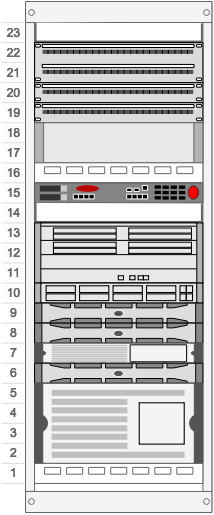
\includegraphics[]{fig2}
	\caption{Exemplo de figura sem escala}
	\label{fig2}
\end{figure}

Você pode rotacionar figuras também. Para isso utilize o parâmetro angle=-90. Repare que a escala da figura foi modificada pelo parametro height. Você também pode utilizar scale

\begin{figure}
	\centering
	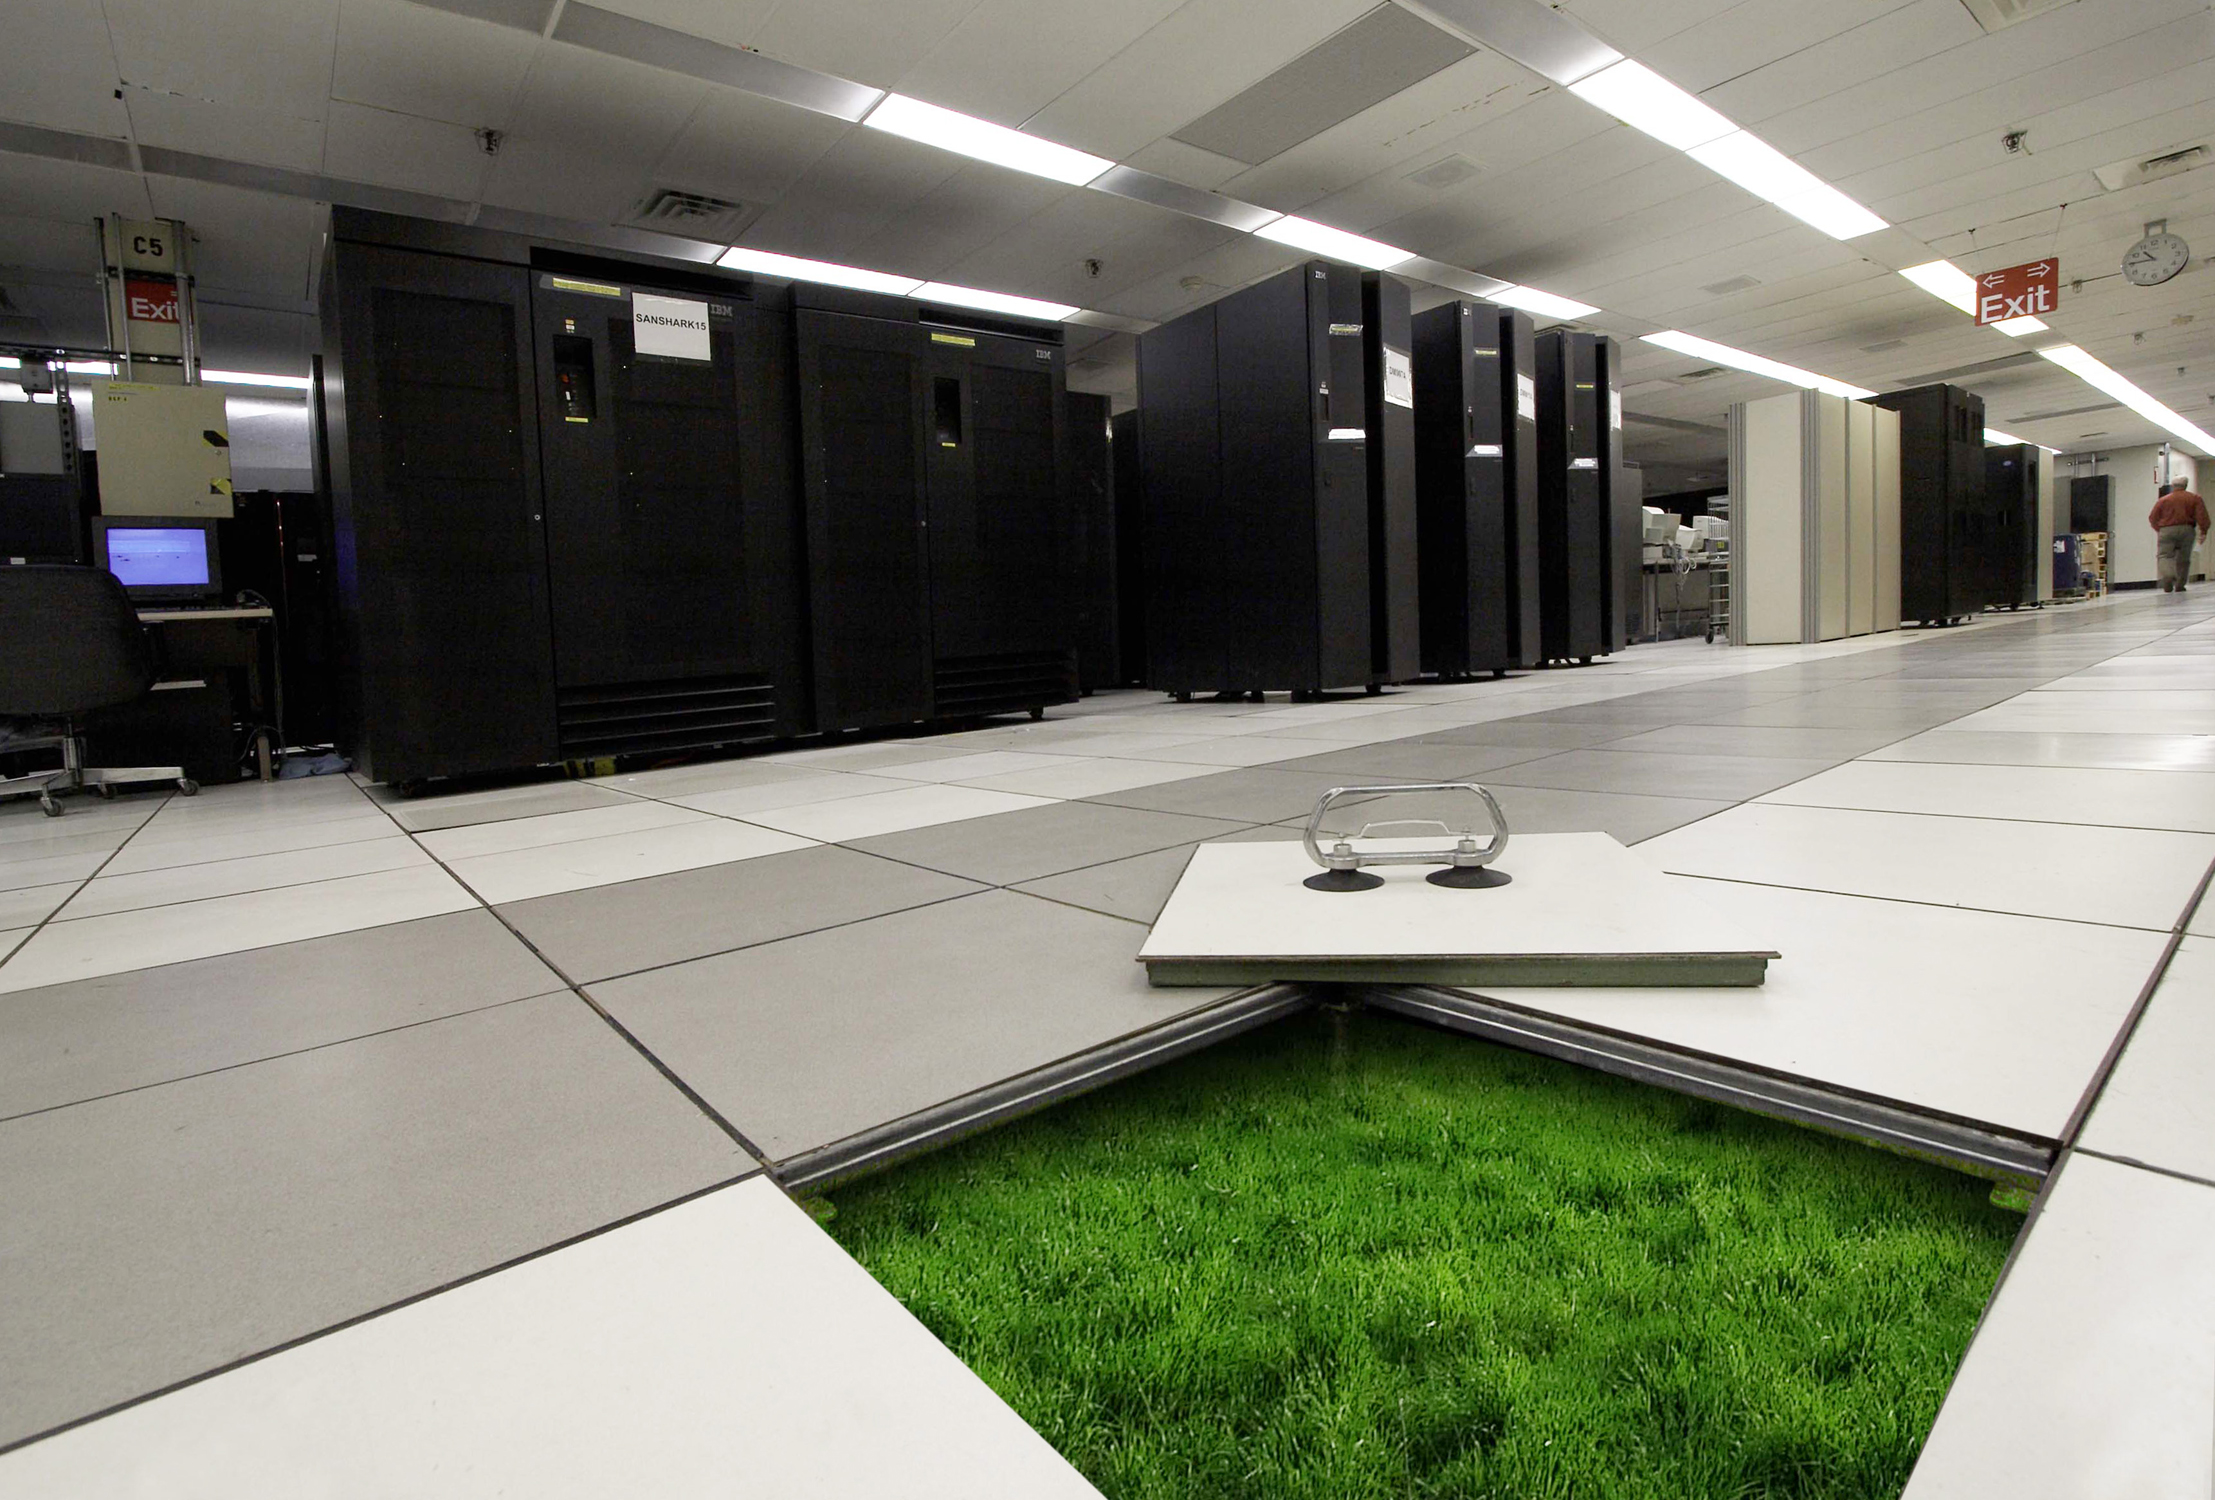
\includegraphics[height=\textwidth,angle=-90]{fig3}
	\caption{Exemplo de figura rotacionada}
	\label{fig3}
\end{figure}


%% ***********************************************************************
%% === ate aqui    =====  ================================================
%% ***********************************************************************

\end{document}